\documentclass[a4paper,12pt]{article}

\usepackage{prettylatex}
\usepackage{titlepage}
\usepackage{float}

\top{Université de Technologie de Belfort-Montbéliard}{}
\title{Gestion des voies ferroviaires}{Projet de LO41}
\author{Maxime \textsc{Brodat} \\ Esia \textsc{Belbachir}}
\date{Semestre de printemps 2016}

\begin{document}

\maketitlepage

\tableofcontents
\pagebreak

%\neverindent

\section{Fonctionnement global}

Le programme fonctionne de la manière suivante : il prend en argument un nom de fichier contenant la liste des trains à lancer dans le système et lit ce fichier comme une partition. Au terme du programme, tous les trains doivent avoir passé le réseau de chemin de fer.

\subsection{3 processus}

\subsubsection{Main}

Le processus main est celui qui va lancer tous les autres processus et s'occuper de la terminaison du programme. Notamment, il s'occupe du processus train, du processus manager, et de la coordination des interruption (SIGINT) à l'échelle du programme entier.

\subsubsection{Train}

C'est le processus train qui va être responsable de lire le fichier des trains et de gérer le comportement de chacun. Ce processus se compose d'une tread par train et de la thread principale qui encadre les autres.

\subsubsection{Manager}

Le processus manager est responsable des décisions d'aiguillage des trains dans le sytème. Il est composé d'une thread principale et de 3 thread secondaires aiguillage 1, aiguillage 2 et tunnel. Chacune des 3 threads secondaires est responsable de l'autorisation de passage des trains sur leur zone critique.

\subsection{Initialisation, interruption et terminaison}

Si l'initialisation du programme se déroule normalement (pas d'interruption extérieure), le processus principal récupère le nom du fichier de trains à lire, rattache un handler particuler pour les signaux SIGINT (voire plus loin), crée une file de message (communication inter-processus), crée les processus manager et train et se met en attente du processus train.

Lorsque le processus train se termine (tous les trains sont passés), celui-ci se termine de lui même. Le processus principal est alors chargé d'envoyer un signal d'interruption au processus manager qui va alors se terminer proprement. Enfin, la file de message inter-processus est supprimée et le programme se termine.

Le programme est capable de gérer les interruptions (SIGINT) envoyées au processus main et de terminer le programme sans qu'il n'y ai de fuite mémoire. Le processus main est équipé d'un handler de SIGINT qui s'occupe de propager l'information d'interruption aux processus manager et train sous forme de signaux SIGINT. Ensuite, le programme se termine de la même manière qui s'il n'y avait pas eu d'interruption (attente des processus train et manager, et suppression de la file de message inter-processus).

\subsection{Communication inter-processus}

Les threads du processus train et les threads du processus manager ont besoin de communiquer entre elles pour coordonner les passages de train. Cette communication se met en place sous forme d'une file de message.

Un message contient les informations suivantes :
\begin{itemize}
	\item Les identifiants du destinataire et de la source : Les trains ont des identifiants supérieurs ou égaux à 10 car les identifiant de 1 à 9 sont réservés pour des threads particulières qui requièrent des valeurs statiques (aiguillage 1, aiguillage 2 et tunnel par exemple ont les identifiants 1, 2, et 3).
	\item Le type de message : requête, autorisation ou notification. Une requête est une demande de passage addressée à une zone critique. Une autorisation est une réponse d'une zone critique à un train pour l'informer qu'il a la permission de passer. Une notification est envoyée d'un train à une zone critique ; elle informe la zone critique que le train à quitté la voie en question.
	\item Des informations sur le train lorsque que celui-ci est la source du message.
\end{itemize}

\subsection{Fonctionnement global simplifié}

\begin{figure}[H]
	\centering
	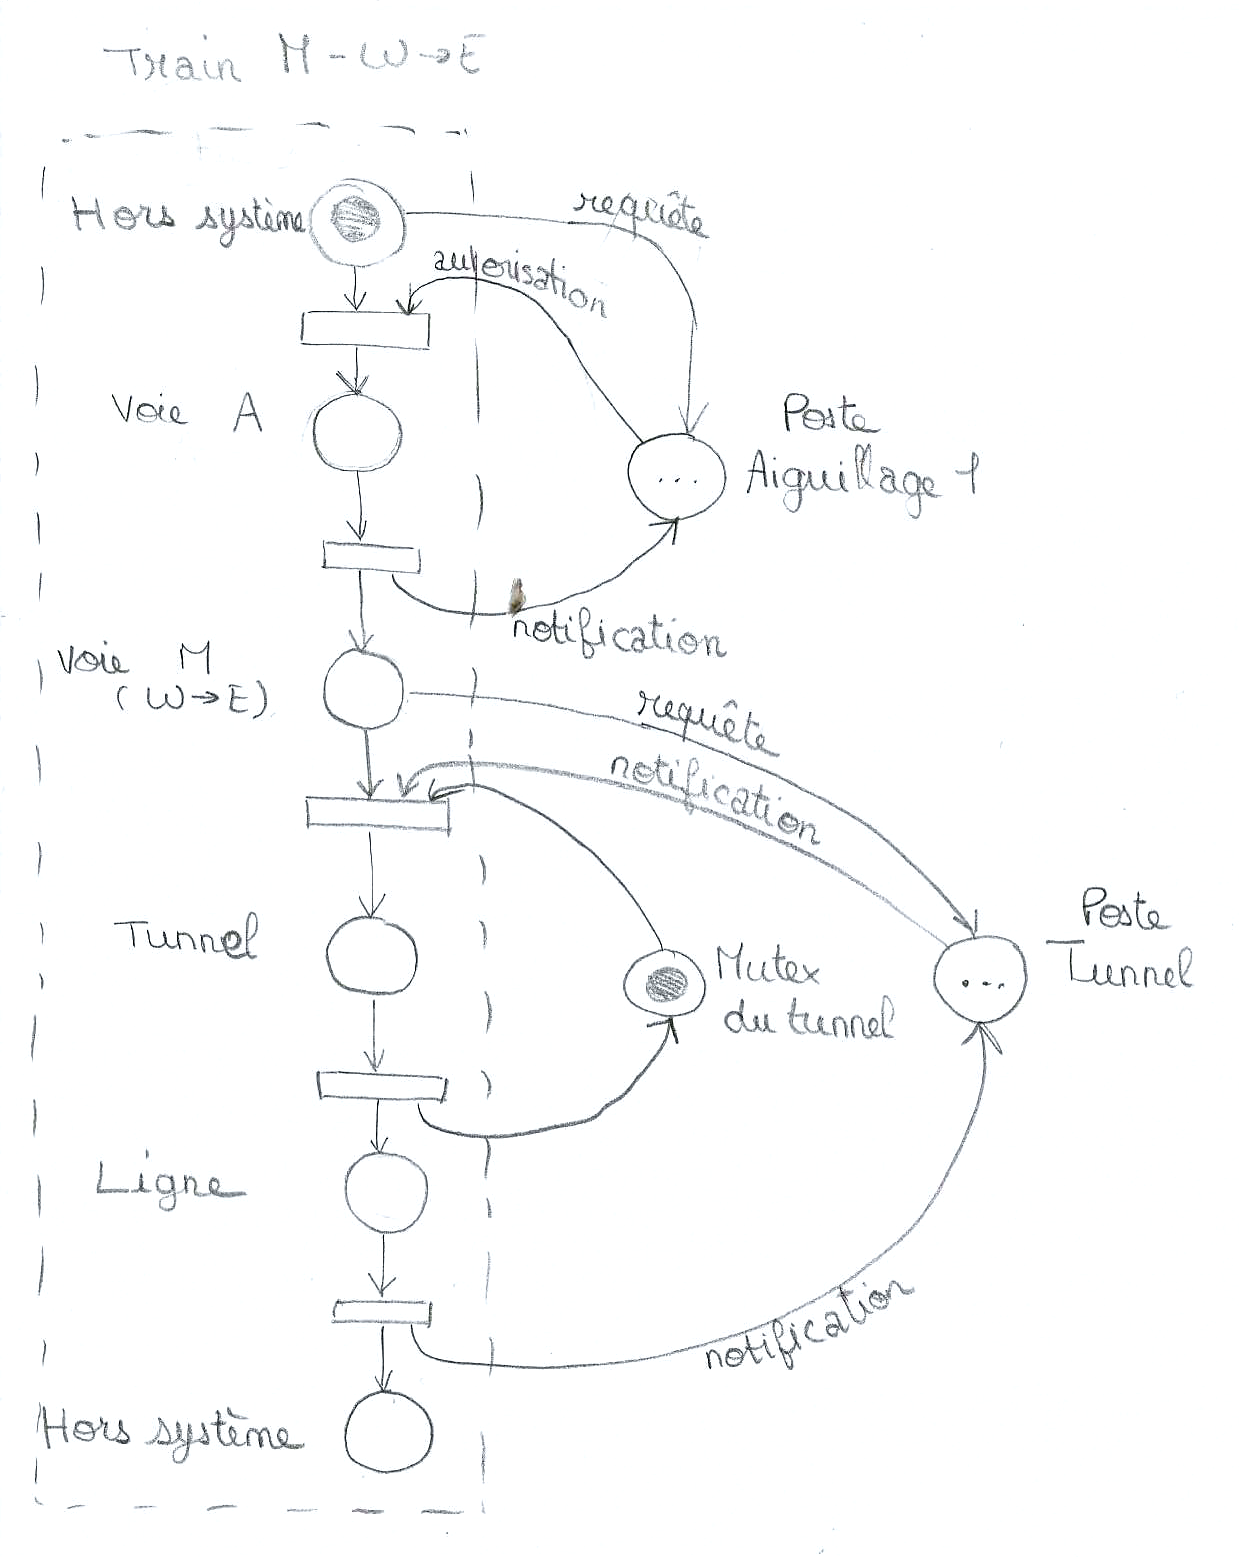
\includegraphics[scale = 0.65]{img/reseau_petri.png}
	\caption{Réseau de Petri appliqué au cas des trains de marchandise dans le sens W $\rightarrow$ E}
\end{figure}


\section{Le processus train}

\subsection{Initialisation, interruption et terminaison}

La fonction principale du processus train prend en argument le nom du fichier de trains à lire. Elle va ensuite mettre en place un handler pour SIGINT qui informe les threads de la terminaison imminante du programme, les attend et permet de libérer toutes les ressources allouées. Ensuite, il initialise un Parser qui permet de lire, train par train, les caractéritiques des trains qui doivent être envoyées dans le système. Afin de conserver les identifiants des threads de trains qui vont être lancées, un tableau est alloué à la taille indiquée dans le fichier. Ensuite, chaque train est lancée au moment indiqué dans le fichier (voire paragraphe suivant). Si une erreur de lecture se produit, le train qui était alors en train d'être lancé est abandonné et le programme passe directement au train suivant.

Le fichier se compose de la manière suivante :

\begin{itemize}
	\item 1er ligne : <nombre de trains n>
	\item n lignes suivantes : <moment du lancement> <type de train> <sens de circulation>
\end{itemize}

Le moment du lancement du train correpond à un nombre de secondes après le début du programme. Les trains doivent être classés dans l'ordre croissant de leur lancement.

Lorsque tous les trains sont lancées, la thread principale du processus train se met en attente de toutes ses threads de trains ou d'un signal d'interruption SIGINT. Si un signal SIGINT est reçu, un signal SIGTERM est envoyé à toutes les threads de trains.

\subsection{Les threads du processus train}

Chaque thread de train a un comportement prédéfini en fonction de son type (Marchandise, Grande Ligne ou TGV) et de sa direction (est-ouest ou ouest-est). Cependant, ils ont un certain nombre de comportements communs :
\begin{itemize}
	\item Tous les trains sont considérés comme en dehors du sytème à leur démarrage lorsqu'ils proviennent de l'est ou de la voie A. Il doivent recevoir une autorisation de la zone critique la plus proche pour entrer dans le système.
	\item Lorsqu'un train arrive aux abord d'une zone critique, il s'arrête et envoie une requête à la zone critique en question au travers de la file de message inter-processus.
	\item Après avoir quitté une zone critique, le train envoie une notification au manager responsable de la zone critique.
	\item Les trains doivent recevoir une autorisation et aquérir un mutex pour passer le tunnel afin qu'il n'y ait qu'un seul train à la fois dans le tunnel.
	\item Une thread de train se termine d'elle même lorsque le train quitte le système.
\end{itemize}

\section{Le processus manager}

\subsection{Initialisation, interruption et terminaison}

Le processus manager ne prend pas d'arguments. Durant l'initialisation, il initialise les 5 compteurs des zones critiques (qui indiquent le nombre de trains sur la voie en question et le sens du flux de train) et le mutex de protection de ces compteurs. Ensuite, un handler de SIGINT est mis en place de manière à ce que, si un signal SIGINT survient, les trois threads de manager sont terminées et le processus manager se termine. Enfin, les trois threads de manager sont créées et lancées dans leur méthode.

Les 3 threads secondaires du manager ne se terminent jamais d'elles-même car elles sont prisent dans une boucle infinie. Lorsque tous les trains ont fini de passer, le processus manager reçoit un signal SIGINT qui sera alors attrapé et les différentes threads seront terminées proprement par le biais de signaux SIGTERM puis avec la libération de ressources.

\subsection{Les threads du processus manager}

Les 3 threads secondaires du manager (aiguillage 1, aiguillage 2 et tunnel) fonctionnent tous selon la même fonction. En arrivant sur cette fonction, les trois threads vont << se connecter >> à la file de message et effectuer indéfiniement (jusqu'à recevoir un signal de terminaison SIGTERM) les instructions suivantes :

\begin{enumerate}
    \item Récupérer les messages de la file de message qui sont destinés au manager en question.
    \item Traiter toutes les notifications dans l'ordre où elles arrivent et stocker les requêtes dans une liste de messages annexe qui sera traintée plus tard (voire plus bas).
    \item Traiter toutes les requêtes de la liste de messages.
    \item Attend une durée déterminée avant de recommencer ce cycle.
\end{enumerate}

Ainsi, à la fin de chaque itération pour une thread donnée, cette thread a traitée tous les messages de notification et tous les messages de requête qu'il lui était possible d'autoriser.

\subsubsection{Réception et résolution des messages}

La réception des messages de requête se fait par le stockage dans une liste de messages (structure créée pour l'occasion). Celle-ci fonctionne comme une structure de donnée de queue (FIFO).

Les requêtes précédemment stockées dans la liste de message sont lues une par une et les requêtes sont traitées par priorité décroissante (TGV puis GL puis M) et dans l'ordre chronologique (premier arrivé premier servi). Si une requête ne peut donner lieu à une autorisation de passer, elle est remise dans la liste de message pour être traitée ultérieurement.

\section{Améliorations possibles}

Actuellement, les processus ne bloquent jamais les signaux. Il pourrait être intéressant d'ignorer les SIGINT par exemple pendant l'initialisation, dans les handlers et pendant la terminaison des processus (libération des ressources) pour assurer une meilleure robustesse et éviter les appels récursifs dans ces zones de code critiques.

Beaucoup de variables sont stockées en publique, ce qui peut être problématique car tous les processus y ont accès et peuvent donc les modifier. On pourrait penser à des passages par arguments ou par file de message pour réduire le nombre de variable globales.
\end{document}
